\documentclass[10pt,a4paper]{article}
\usepackage[utf8]{inputenc}
\usepackage[german]{babel}
\usepackage[T1]{fontenc}
\usepackage{amsmath}
\usepackage{amsfonts}
\usepackage{amssymb}
\usepackage{float}
\usepackage{graphicx}
\usepackage{listings}
\renewcommand\thesubsection{\alph{subsection}}
\begin{document}

\begin{center}
Regelung dynamischer Systeme: Praktikum 4

Johannes Reidl, Sigurd Sippel
\end{center}

\section{Schwebekugel}
\subsection{Bestimmung von $i_0$ und  $u_o$ im Arbeitspunkt}
\begin{figure}[H]
  \begin{align}
	  m\ddot{x} = mg - C * (\frac{i}{x})^2 \nonumber \\
	  \frac{m\ddot{x} - mg}{-c} = (\frac{i}{x})^2 \nonumber \\
	  \sqrt{\frac{m* (\ddot{x} - g)}{-c} * x} = i \nonumber \\
	  \sqrt{\frac{0,025kg * -9,81\frac{m}{s^2}}{-5 * 10^{-6}\frac{Nm^2}{A^2}}} * 0,015m = i \nonumber \\
	  \underline{\underline{i = 3,322A}} \nonumber
  \end{align}
\end{figure}

\begin{figure}[H]
  \begin{align}
	  u(t) = R * i(t) + L * \underbrace{\frac{di(t)}{dt}}_\text{0, da Kugel in Ruhe} \nonumber \\
	  u(t) = 3\frac{V}{A} * 3,322A = \underline{\underline{9,966V}} \nonumber
  \end{align}
\end{figure}


\subsection{Strukturbilder der DGLn}
\begin{figure}[H]
	\centering
	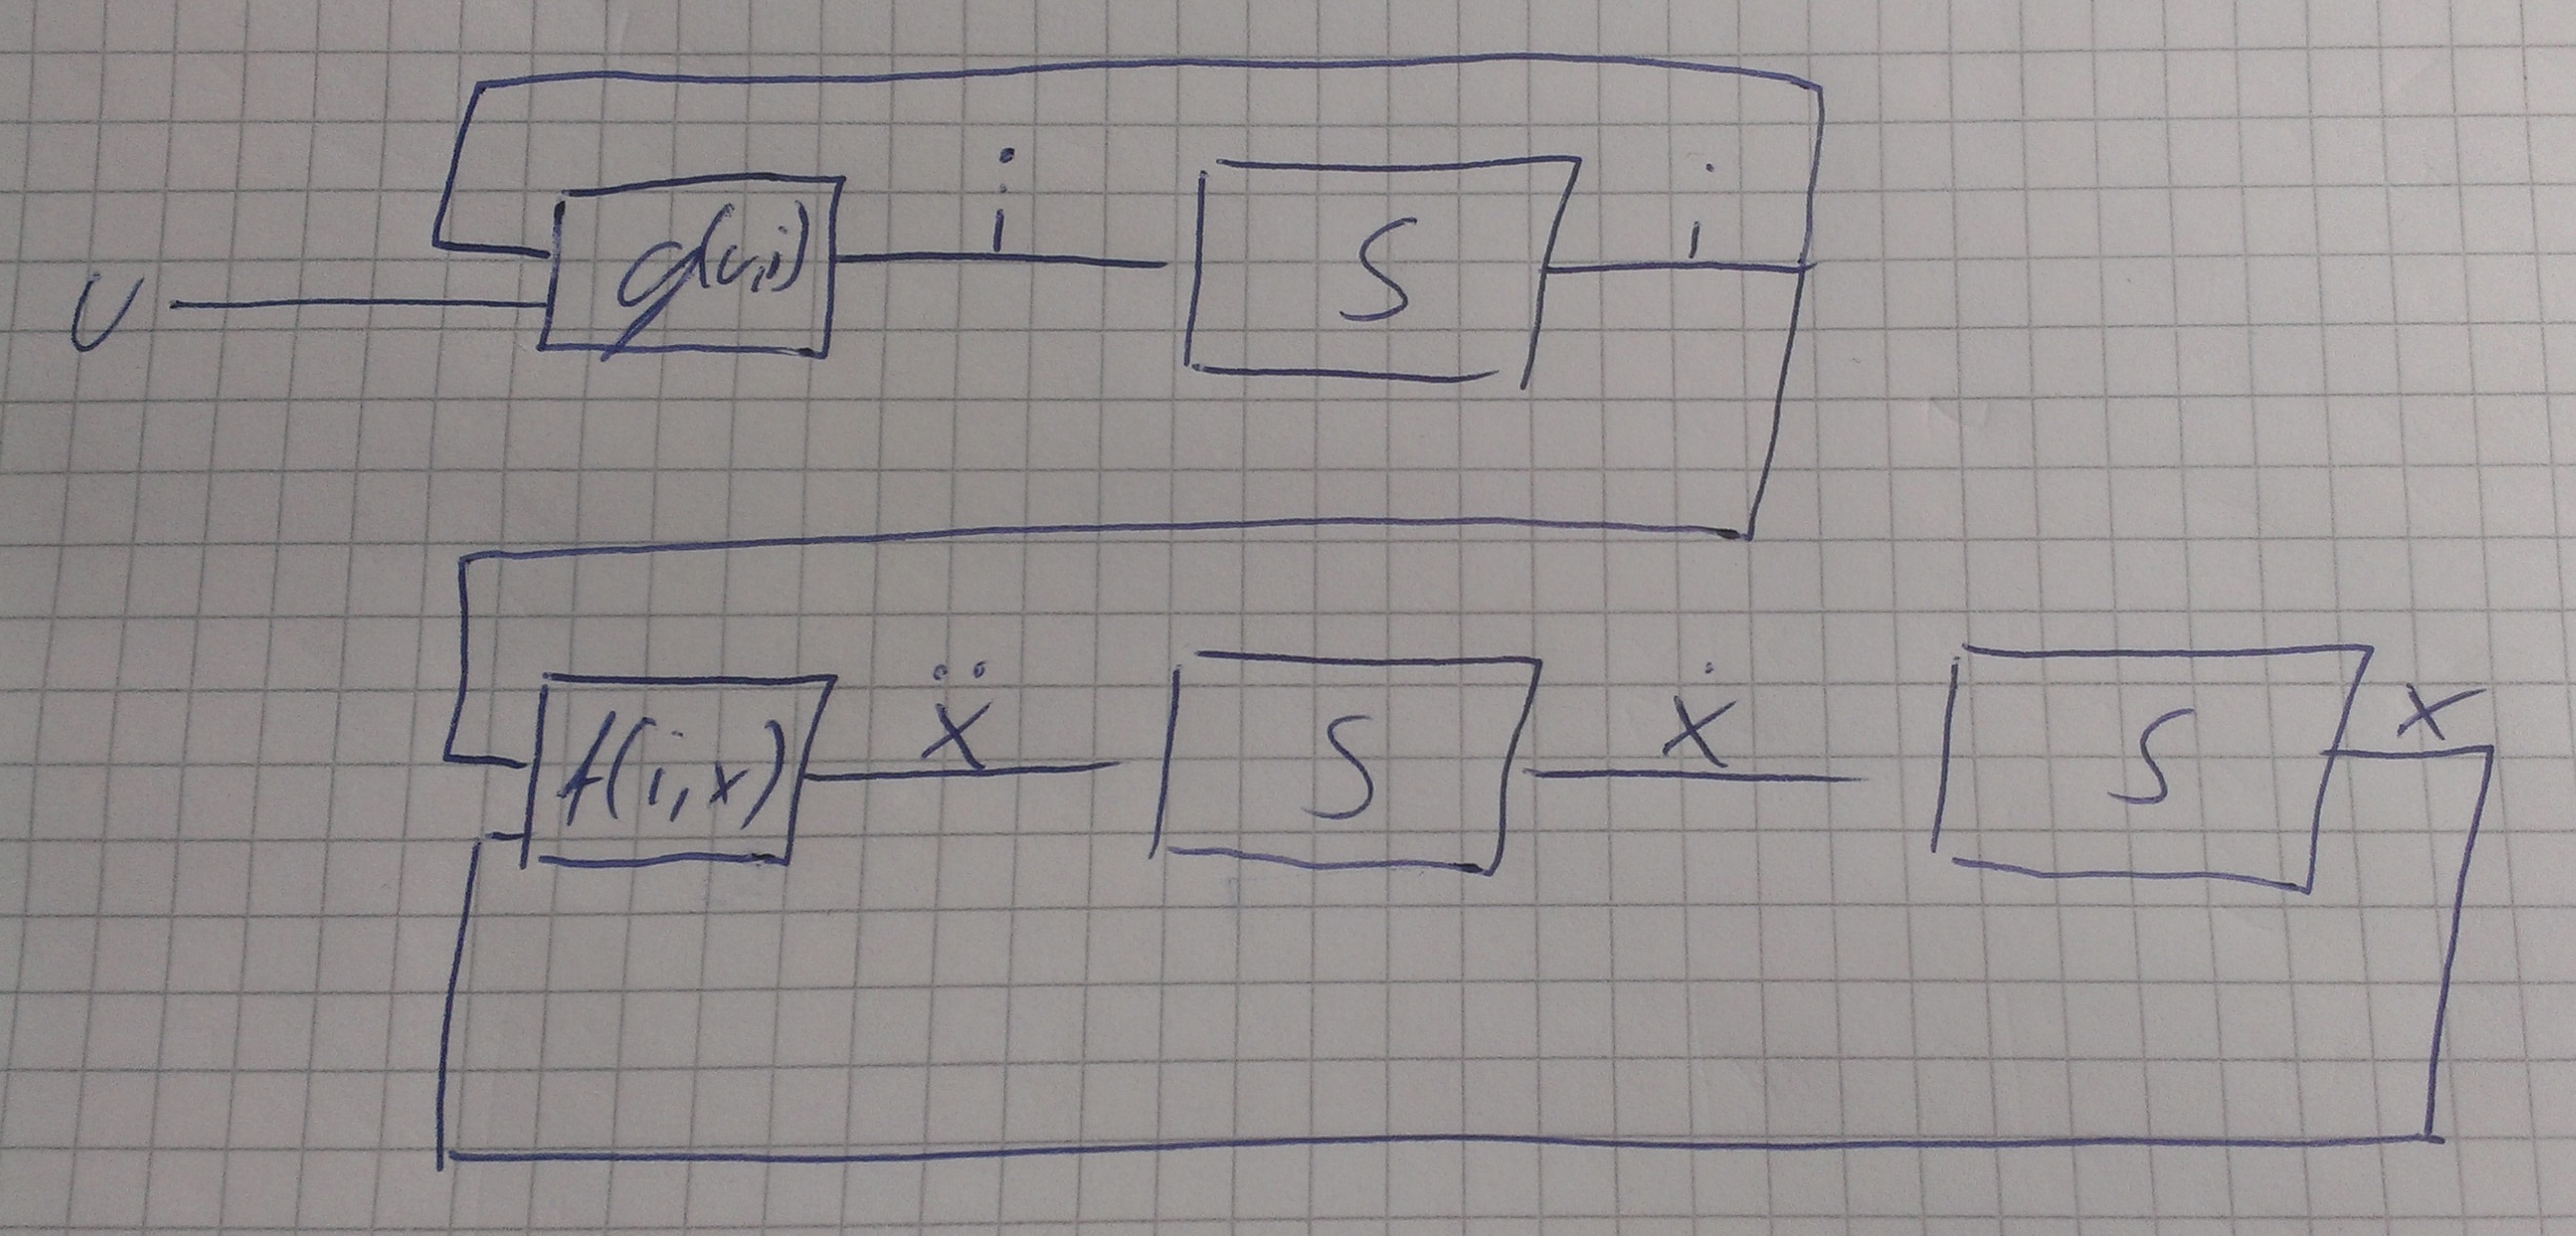
\includegraphics[width=1\textwidth]{screens/schaltbild.jpg}
	\caption{Strukturbild der DGLn}
\end{figure}


\subsection{Linearisierung}
\begin{figure}[H]
  \begin{align}
	  \frac{\partial g}{\partial u} \Big|_A = \frac{1}{L} \nonumber \\
	  \frac{\partial g}{\partial i} \Big|_A = -\frac{R}{L} \nonumber \\
	  \frac{\partial f}{\partial i} \Big|_A = -1,77778\frac{m}{A^2s^2} * i_0 \nonumber \\
	  \frac{\partial f}{\partial x} \Big|_A = \frac{0,00441427\frac{m^2}{s^2}}{{x_0}^3} \nonumber \\
	  \Delta \dot{i} = 10\frac{A}{Vs}\Delta u - 30 \frac{m}{s} \Delta i \nonumber \\
	  \Delta \ddot{x} = -5,9\frac{m}{As^2} \Delta i + 1306,4 \frac{1}{s^2} \Delta x \nonumber
  \end{align}
\end{figure}


\subsection{Normieren der linearisierten DGLn auf SI-Größen}
\begin{figure}[H]
  \begin{align}
	\Delta \hat{\ddot{x}} * \Delta \ddot{x}_N = -5,9\frac{m}{As^2} * \Delta \hat{i} \Delta i_N + 1306,4 \frac{1}{s^2} \Delta \hat{x} * \Delta x_N \nonumber \\
	\Delta \hat{\ddot{x}} = -5,9\frac{m}{As^2} * \Delta \hat{i} * \frac{\Delta i_N}{\Delta \ddot{x}_N} + 1306,4 \frac{1}{s^2} \Delta \hat{x} * \frac{\Delta x_N}{\Delta \ddot{x}_N} \nonumber \\
	\Delta \hat{\ddot{x}} = -5,9\frac{m}{As^2} * \Delta \hat{i} * \frac{m}{As^2} * \frac{A}{\frac{m}{s^2}} + 1306,4 \frac{1}{s^2} \Delta \hat{x} * \underbrace{\frac{1}{s^2} * \frac{mm}{\frac{m}{s^2}}}_\text{$\frac{mm}{m} = \frac{1mm}{1000mm} = 10^{-3}$} \nonumber
  \end{align}
\end{figure}


\subsection{Übertragungsfunktionen}
\begin{figure}[H]
  \begin{align}
	  \Delta\ddot{x} = -5,9\Delta i + 1306,4 \Delta x \nonumber \\
	  5,9
  \end{align}
\end{figure}



\subsection{Gesamtübertragungsfunktion der Regelstrecke}
\begin{figure}[H]
  \begin{align}
	  G(s) = G_1(s) * G_2(s) \nonumber \\
	  = \frac{59 * (-1)}{(-s^3 -20s^2 + 1306,4s + 39192) * (-1)} \nonumber
  \end{align}
\end{figure}

\end{document}
